%!TEX root = ../../thesis.tex

\section{RV precision update}
\label{sec:rv_precision_values}

\begin{figure}
    \centering
    \begin{tabular}{cc}
        \multicolumn{2}{c}{\citet{figueira_radial_2016}}\\
        \multicolumn{2}{c}{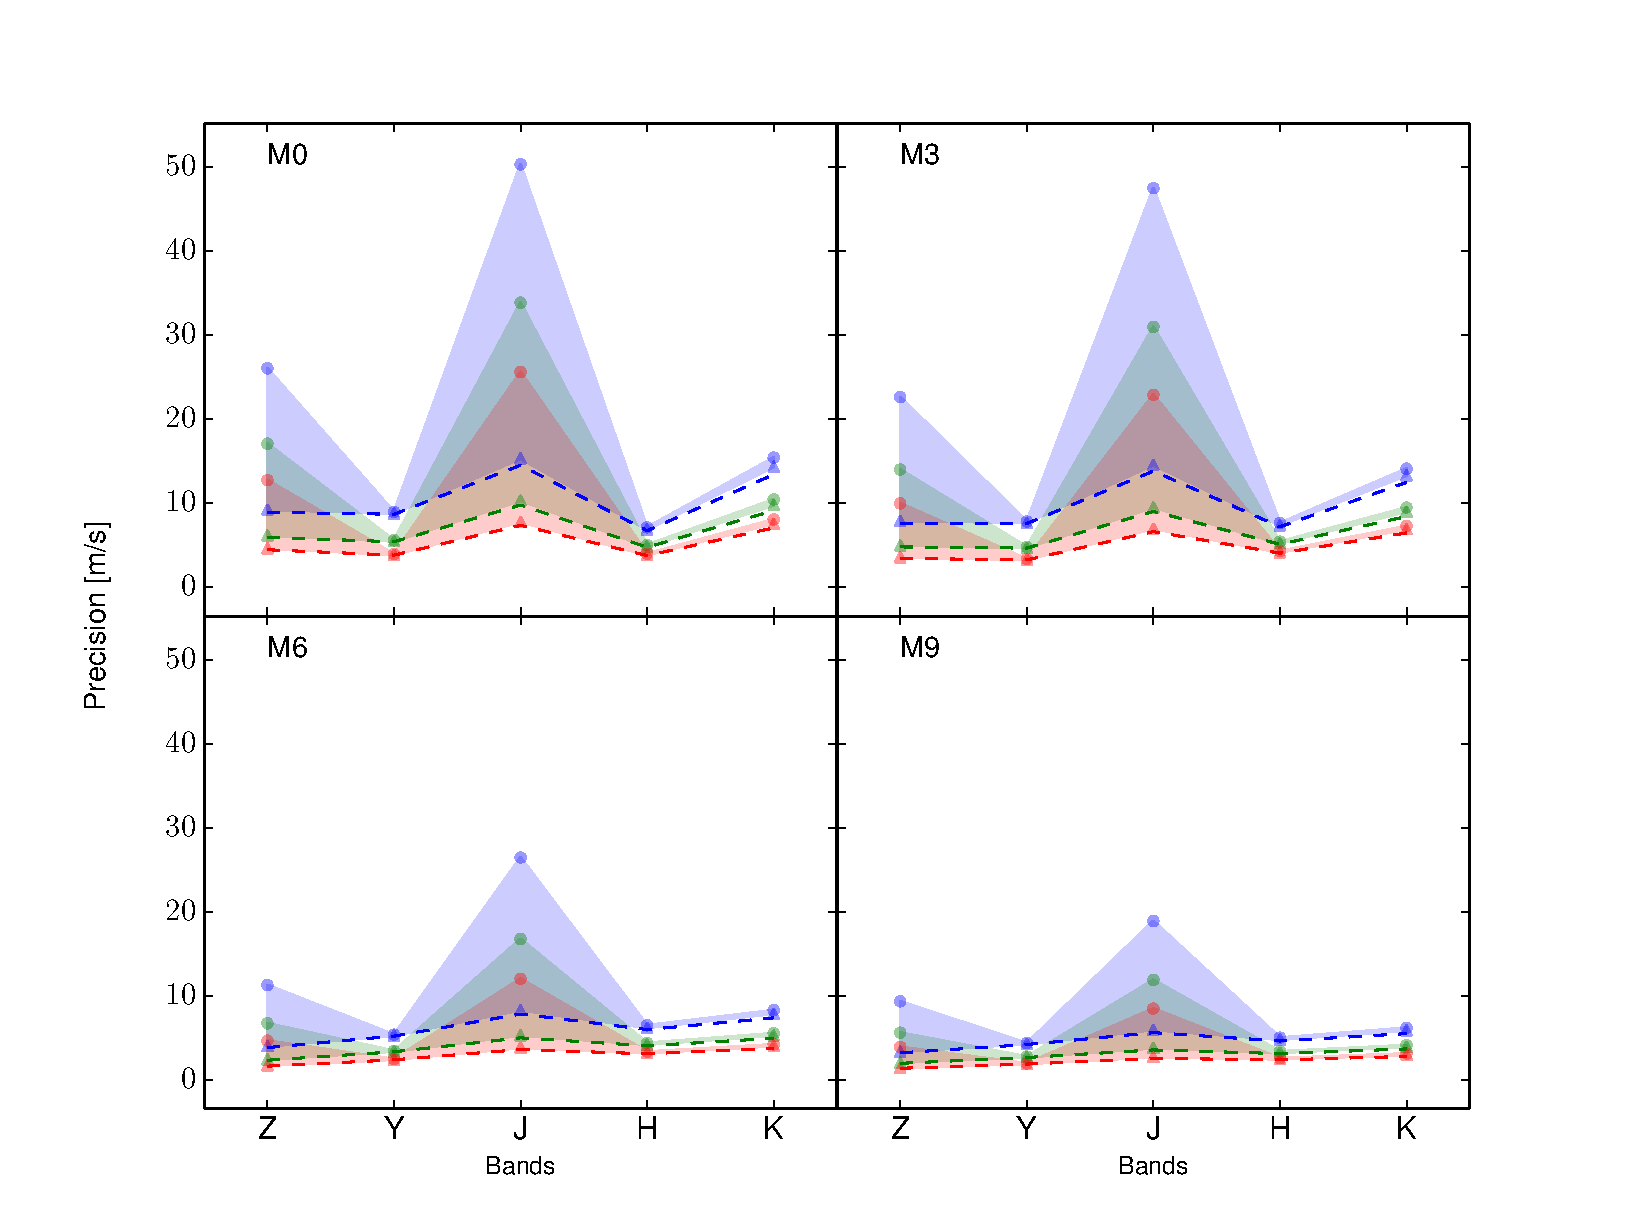
\includegraphics[width=0.48\linewidth]{figures/information-content/Rvprec_vsini1.pdf}}\\
        {PHOENIX-ACES} & {BT-Settl}\\
        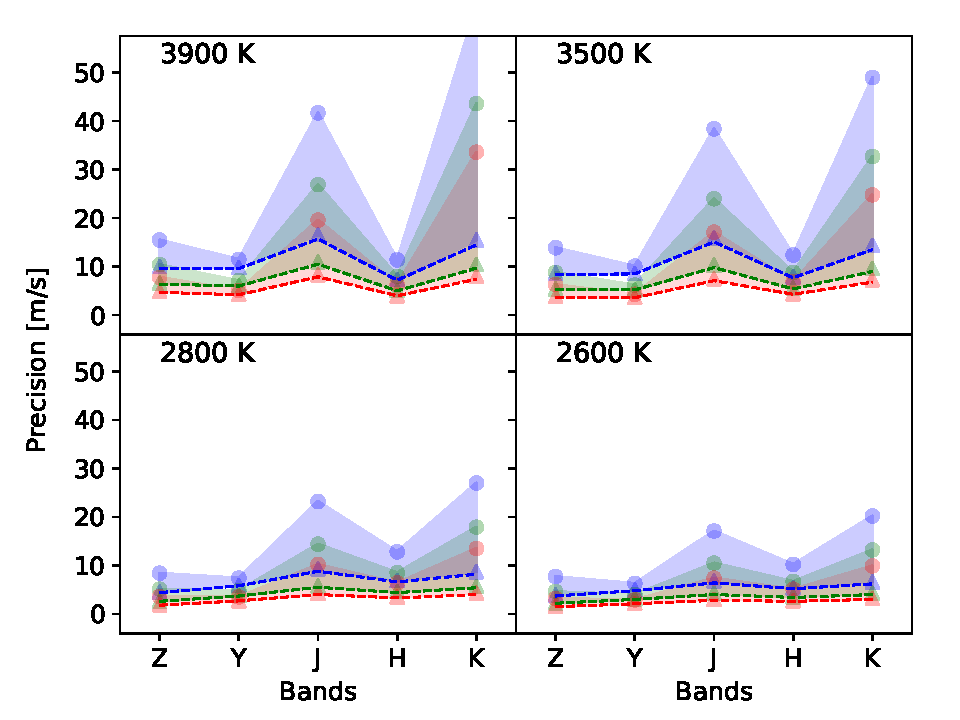
\includegraphics[width=0.47\linewidth]{figures/information-content/aces_4panel} &
        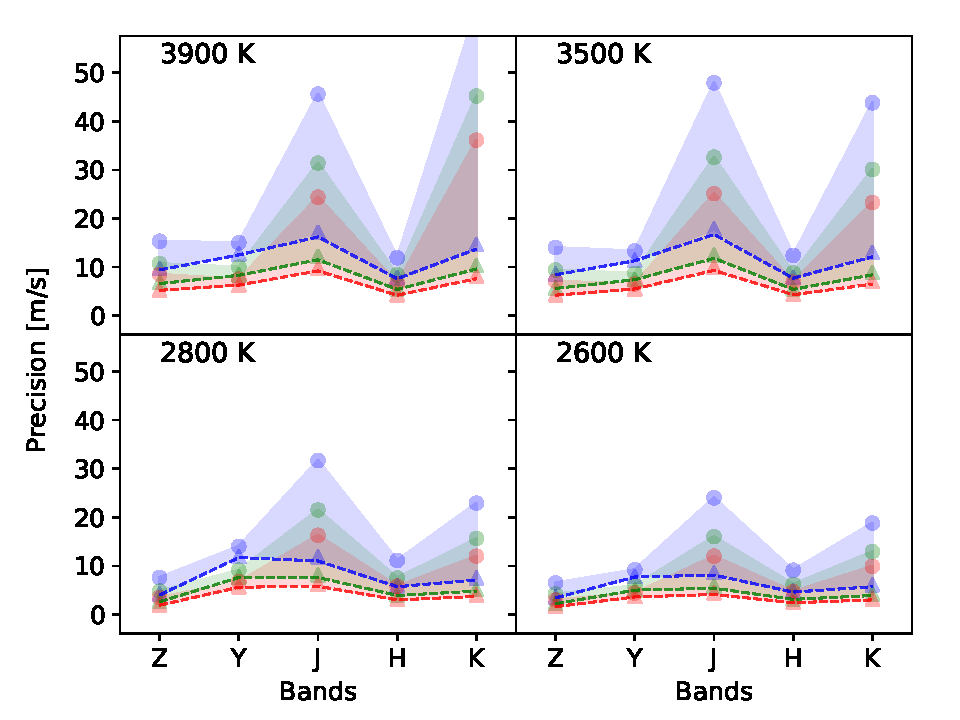
\includegraphics[width=0.47\linewidth]{figures/information-content/btsettl_4panel} \\
    \end{tabular}
    \caption[Comparision of {RV} precision results to~\citet{figueira_radial_2016}.]{Comparison of the updated precision values to the original values.
        Top: Figure~1 from~\citet{figueira_radial_2016}.
        Bottom: Updated precision values computed using \eniric{} using the {PHOENIX-ACES} (left) and the {BT-Settl} (right) models.
        Each panel shows the precision achieved as a function of spectral band for stars with a rotational velocity of \Vsini=1.0\kmps{} and spectral types {M0}~(3900\K), {M3}~(3500\K), {M6}~(2800\K), and {M9}~(2600\K{}).
        The dashed line represents the theoretical limits imposed by Condition~\#1, and the filled area represents the values within the limits set by Conditions~\#2 (circles) and \#3 (triangles); blue, green, and red represent the results obtained for resolutions of 60\,000, 80\,000, and 100\,000, respectively.
        The spectra were normalized to have a \snr{} of 100 per resolution element as measured at the centre of the \emph{J}-band.}
    \label{fig:figueria_comparision}
\end{figure}

As detailed in the \cref{sec:eniric} updating the software introduced several changes that affect the {RV} precisions values slightly, the numerical gradient, and the masking order for Condition~\#2 and more importantly the bug also found with Condition~\#2.

The 180 spectral combinations from~\citet{figueira_radial_2016}, are repeated here using \eniric{} to have an updated and corrected table of relative {RV} precisions.
This table is given in \cref{tab:rv_aces_btsettl}, calculated using the {PHOENIX-ACES} spectra and also the {BT-Settl} models.
 
The precision changes are visually represented in \cref{fig:figueria_comparision} by comparing Figure~1 of~\citet{figueira_radial_2016} (top) to the updated precisions using \eniric{} with the {PHOENIX-ACES} (bottom-left) and {BT-Settl} (bottom-right) models.
Each panel shows the precision achieved as a function of spectral band for stars with a rotational velocity of \Vsini=1.0\kmps{} and spectral types {M0}~(3900\K), {M3}~(3500\K), {M6}~(2800\K), and {M9}~(2600\K).
The dashed line represents the theoretical limits imposed by Condition~\#1, and the filled area represents the values within the limits set by Conditions~\#2 (circles) and \#3 (triangles); blue, green, and red represent the results obtained for resolutions of 60\,000, 80\,000, and 100\,000, respectively.
The spectra were normalized to have a \snr{} of 100 per resolution element as measured at the centre of the \emph{J}-band.

The values for Condition~\#1 and \#3 only have small differences which is barely noticeable, while Condition~\#2 has large band dependant changes, shown by the change in the shaded areas.
For example note that \emph{Z} and \emph{J}-band {RV} precisions decrease with the new results, while the \emph{K}-band gets substantially worse.
This occurs because the software did not mask many of the regions affected by telluric lines, where as in the new results, a significant portion is masked out due to the overlap of telluric lines, leading to a higher \(\delta V_{\rms}\) value.
The \emph{H}-band also sees a small increase in \(\delta V_{\rms}\).

As stated previously the discovery of the bug affecting telluric masking does not change the conclusions of~\citet{figueira_radial_2016}.
These updated {PHOENIX-ACES} values will be published in an upcoming work as an amendment to the~\citet{figueira_radial_2016} values.

In comparing the bottom two panels between the {PHOENIX-ACES} and {BT-Settl} models, there are only small differences, most identifiable in the Condition~\#2 values of the \emph{J}-band.
This shows again that the {PHOENIX-ACES} and {BT-Settl} models are fairly consistent.
This was also visually observed in \cref{subsec:phoenix_comparision}.


\section{Metallicity and \texorpdfstring{\Logg{}}{Logg}}
\label{sec:metallicity_logg}
\begin{figure}
    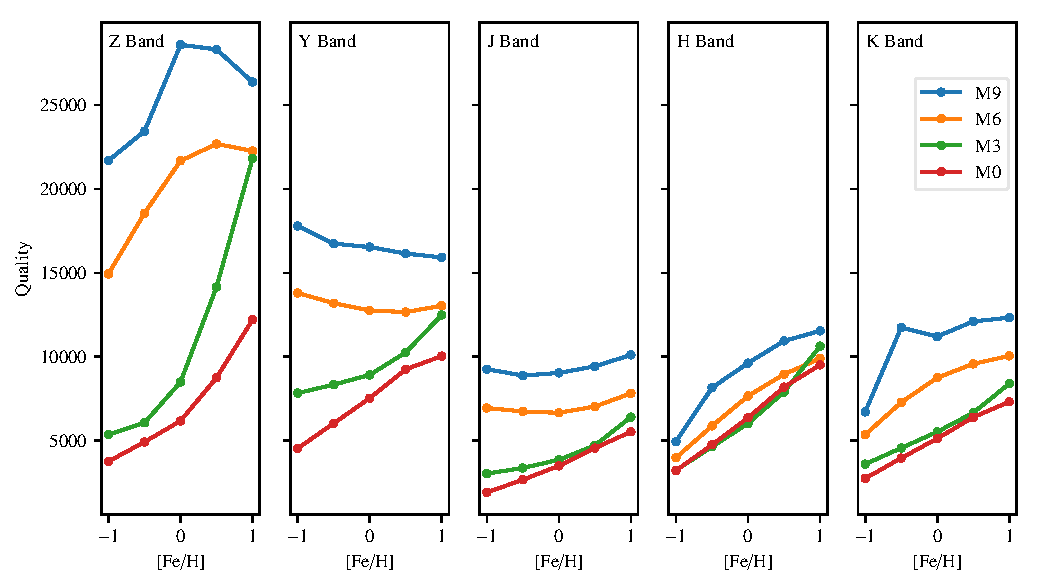
\includegraphics[width=0.95\linewidth]{figures/information-content/metalicity_effect.pdf}\\
    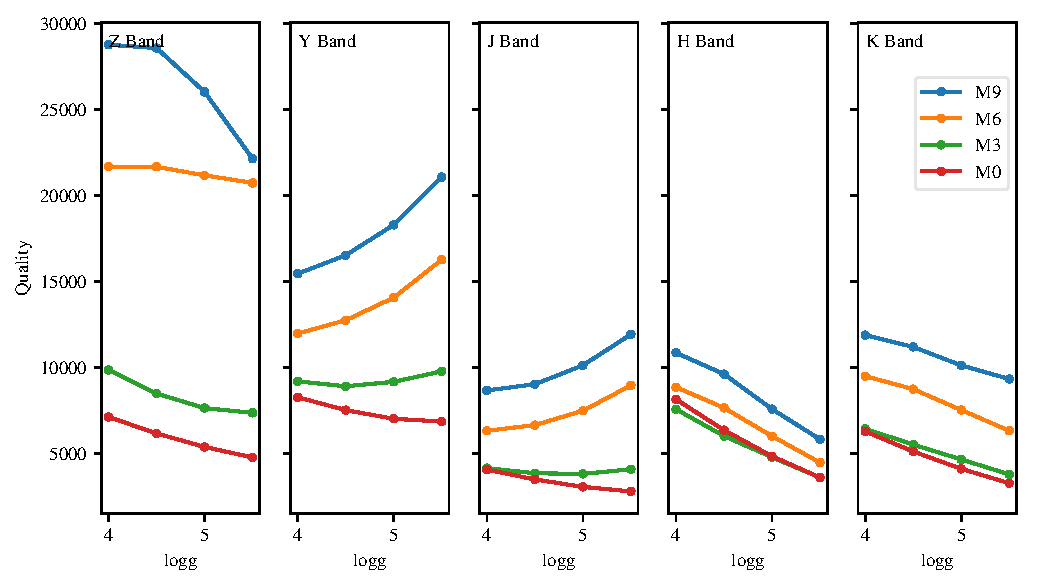
\includegraphics[width=0.95\linewidth]{figures/information-content/logg_effect.pdf}
    \caption[Quality factor verse \feh{} and \Logg{} for different spectral types and wavelength bands.]{Quality factor changes across spectral type and bands for variations in \feh{} and \Logg{}.
        Broadening values are R=100\,000 and \Vsini{}=1.0\kmps{}.
        Top: Quality factor variation of \feh{} between -1.0 to 1.0 at a fixed \Logg{}=4.5.
        Bottom: Quality factor variation of \Logg{} between 4 and 5.5 with fixed \feh{}=0.0.
        Note a higher quality factor corresponds to an increased {RV} precision.}
    \label{fig:logg_metalicity_deviations}
\end{figure}

With the ability to explore a wider range of parameters the range of {PHOENIX-ACES} models were extended to explore the affect of \Logg{} and \feh{} on the relative {RV} precision.
Remember that \Logg{} is a measure of the stellar surface gravity, the gravitational acceleration at the equator expressed in {cgs} units of \si{\centi\metre\per\second\squared} then taking the logarithm of base-10.
The surface gravity is \(g \propto \frac{M}{R^{2}}\) so larger \Logg{} values correspond to stars with smaller radii.
While the metallicity, \feh{}, is a measure of the abundance of elements heavier than Hydrogen and Helium, it is often measured as the ratio of Iron to Hydrogen relative to the Sun.
That is a \feh{}=0 has the same metal ratio as the Sun, a positive \feh{} has more metals, and a negative \feh{} has less metals than the Sun.
The higher abundance of metals creates stronger absorption lines.

\Eniric{} was used to compute the spectral quality factor, \(Q\) (\cref{eqn:quality_factor}), and {RV} precision for all {PHOENIX-ACES} models with \Logg{} between 4.0--5.5 and \feh{} between -1--1, inclusive.
The spectral factor is used for the comparison following~\citet{artigau_optical_2018} in which it was used to compare between models, and observed spectra, independent of the flux levels.
Since \(Q\) is inversely proportional to \(\delta V_{\rms}\) a higher \(Q\) is better.

The spectral quality factor variations for the {M-dwarf}s {M0}, {M3}, {M6}, {M9}, with a broadening of R=100\,000 and $\vsini=1.0$\kmps{} across the \nir{} bands is shown in \cref{fig:logg_metalicity_deviations}.
The top row shows the quality for model spectra with a fixed \Logg=4.5 but having a variable \feh{} between -1.0 to 1.0.
The bottom row shows the opposite: a fixed \feh{}=0.0 while the \Logg{} is varied between 4 and 5.5.
The five separate plots in each row represent the \nir{} wavelength bands \emph{Z}--\emph{K} and the four different coloured lines are the different M-dwarfs (blue {M9}, orange {M6}, green {M3}, red {M0}).

Multiple effects are observed in this figure which are identified below, organized into the separate bands.
Note that the cooler M-dwarfs (M6, {M9}) almost consistently have higher spectral quality factors, corresponding to lower \({\delta V_\rms{}}\) (improved relative precision), if observed at the same relative \snr{} level, as can be seen in \cref{fig:figueria_comparision}.

\begin{itemize}
\item \emph{Z}-band\\
The \emph{Z}-band has a large separation in spectral quality due to spectral type, this is because the continuum of the \emph{Z}-band is severely eroded in the spectra of late M's as they cool.
Each spectral type also behaves very differently to a change in \feh{} and \Logg{}.
For {M0} and {M3} there is a small increase with increasing \feh{} below solar metallicity; above solar metallicity the slopes of the lines dramatically increase, especially for {M3} where the quality more than doubles between a \feh{} value of 0.0 to 1.0.
For {M6} and {M9} there is a sharp decrease in quality as \feh{} falls below solar metallicity (0.0).
The quality seems to peak between \feh{}=0.0--0.5 and begins to decrease at higher metallicity.

As \Logg{} increases in the \emph{Z}-band there is a decrease in spectral quality.
There is a consistent and large separation between early and late M's that.
The quality for {M6} is very shallow, while for {M9} the quality is nearly flat for \Logg{}=4.0 and 4.5 but then decreases sharply at higher \Logg{}.

\item \emph{Y}-band and \emph{J}-band \\
The spectral quality in the \emph{Y}-band is interesting, as the quality appears to converge and diverge with increasing \feh{} and \Logg{} respectively.
For {M0} and {M3} there is an increase in quality as the metallicity increases in both bands, while for {M6} and {M9} there is a decrease in quality in the \emph{Y}-band, converging together beyond \feh{}=1.0.
In the \emph{J}-band the {M6} and {M9} are almost flat with a gentle decrease then increase in quality.

For the \Logg{} variation the opposite occurs.
As the \Logg{} increases from 4.0 to 5.5 {M0} has a small gradual decrease in the spectral quality with {M3} remaining relatively flat.
{M6} and {M9} both increase with increasing \Logg{} so overall there is a divergence in the spectral quality at a larger \Logg{} in both bands.

\item \emph{H}-band and \emph{K}-band \\
The \emph{H}-band and \emph{K}-band also have similar patterns between \feh{}, \Logg{} and quality for all spectral types, with only a small change between the different spectral types.
The spectral quality increases fairly consistently as \feh{} increases and decreases with an increase in \Logg{}.
There does however, appear to be one point that looks out of place in the {M9} spectrum with \feh{}=-0.5.
\end{itemize}

Looking at the bigger picture, there is a striking difference in the quality between the bands.
For the {M0} and {M3} spectra the quality mostly stays under 10\,000, apart from a four points in the \emph{Z} and \emph{Y}-bands at high \feh{}.
For the cooler {M6} and {M9} quality values however there is a large contrast between the \emph{Z} and \emph{Y}-bands, which have a much higher quality, and the other three bands which have a similar quality level.

This difference in spectral quality in the \emph{Z}-band becomes apparent when visualizing the spectra.
The \emph{Z}-band and \emph{J}-band spectra for all four spectral types from~\citet{figueira_radial_2016} are reproduced here in \cref{fig:z_and_j_spectra}.
They show flux as a function of wavelength in the \emph{Z}-band (top) and \emph{J}-band (bottom) for a \Vsini{}=1.0\kmps{} and spectral types {M0}, {M3}, {M6}, and {M9} (\textit{top} to \textit{bottom} panels), when seen at a resolution of 100\,000.
The \emph{Z}-band has substantial erosion of the continuum in the {M6} and {M9} spectra, compared to the other spectra, even of the same spectral type.
The higher number of lines in the M8 and {M9} spectra show why the spectral quality is higher.

\begin{figure}
    \centering
    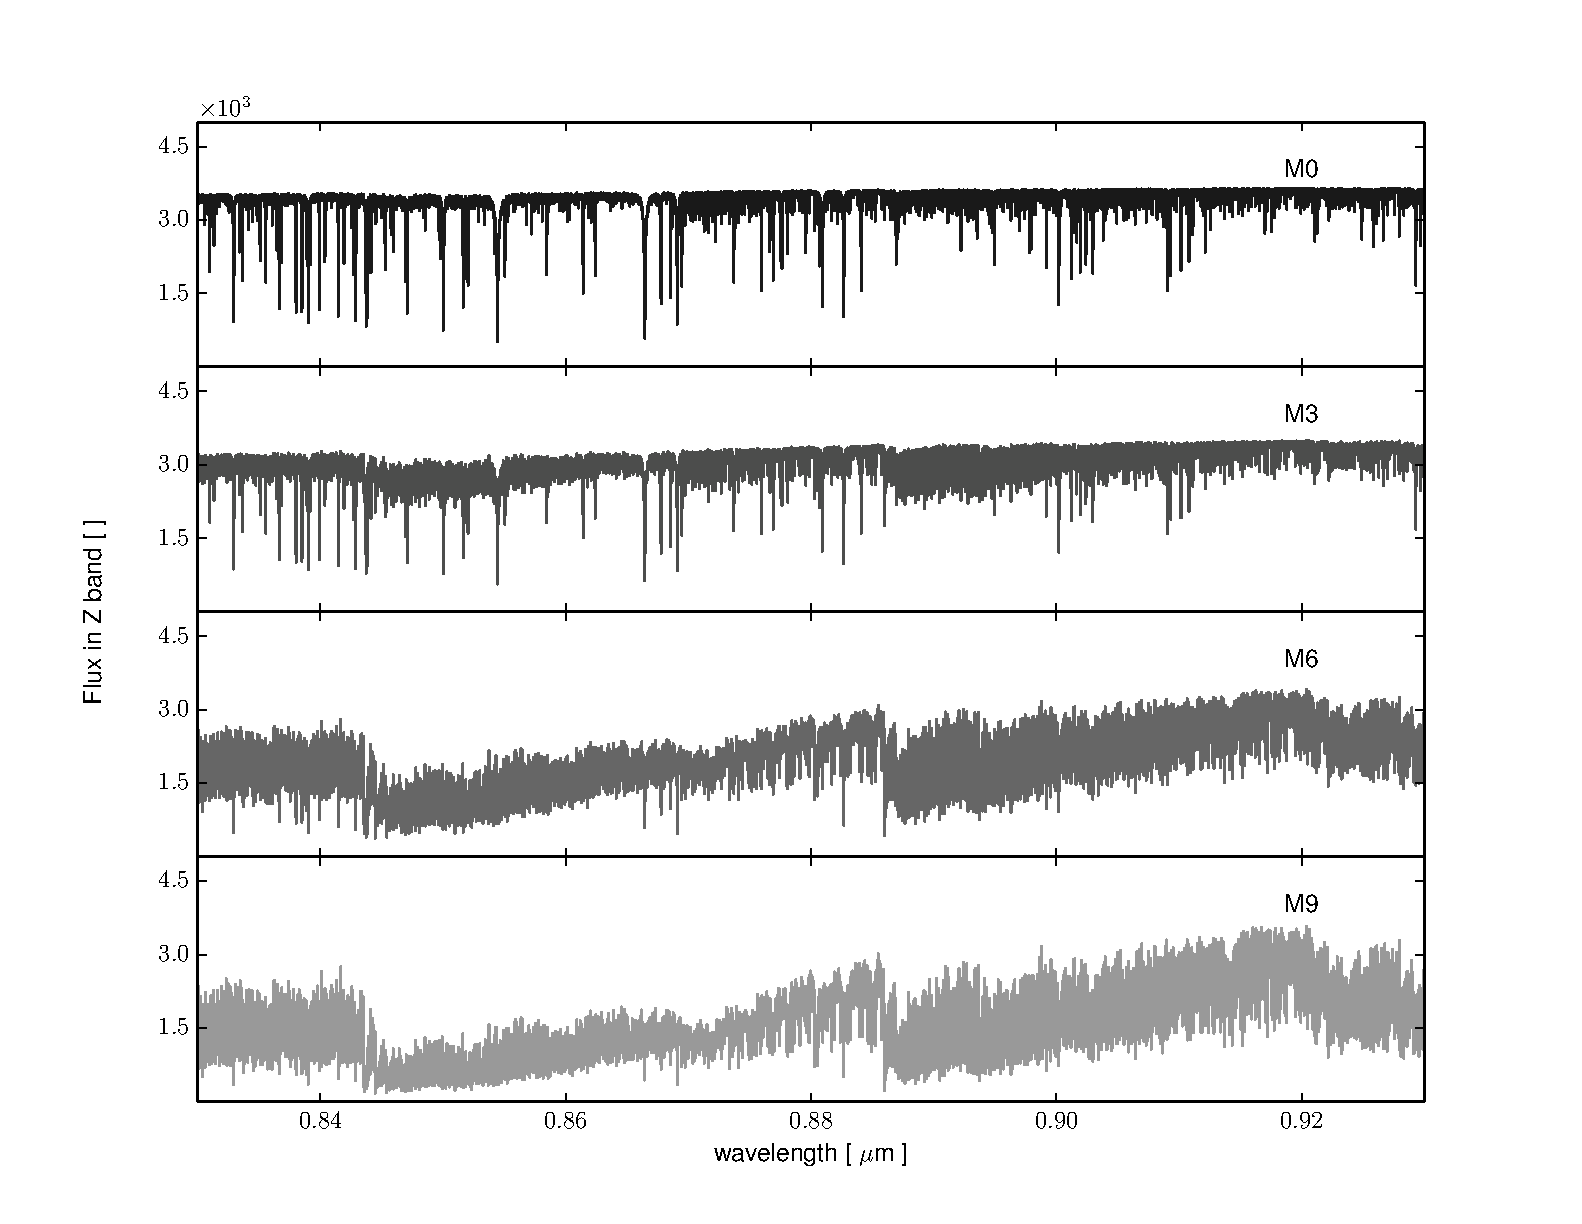
\includegraphics[width=0.78\linewidth]{figures/information-content/figueria_2016_figures/Zband}\\
    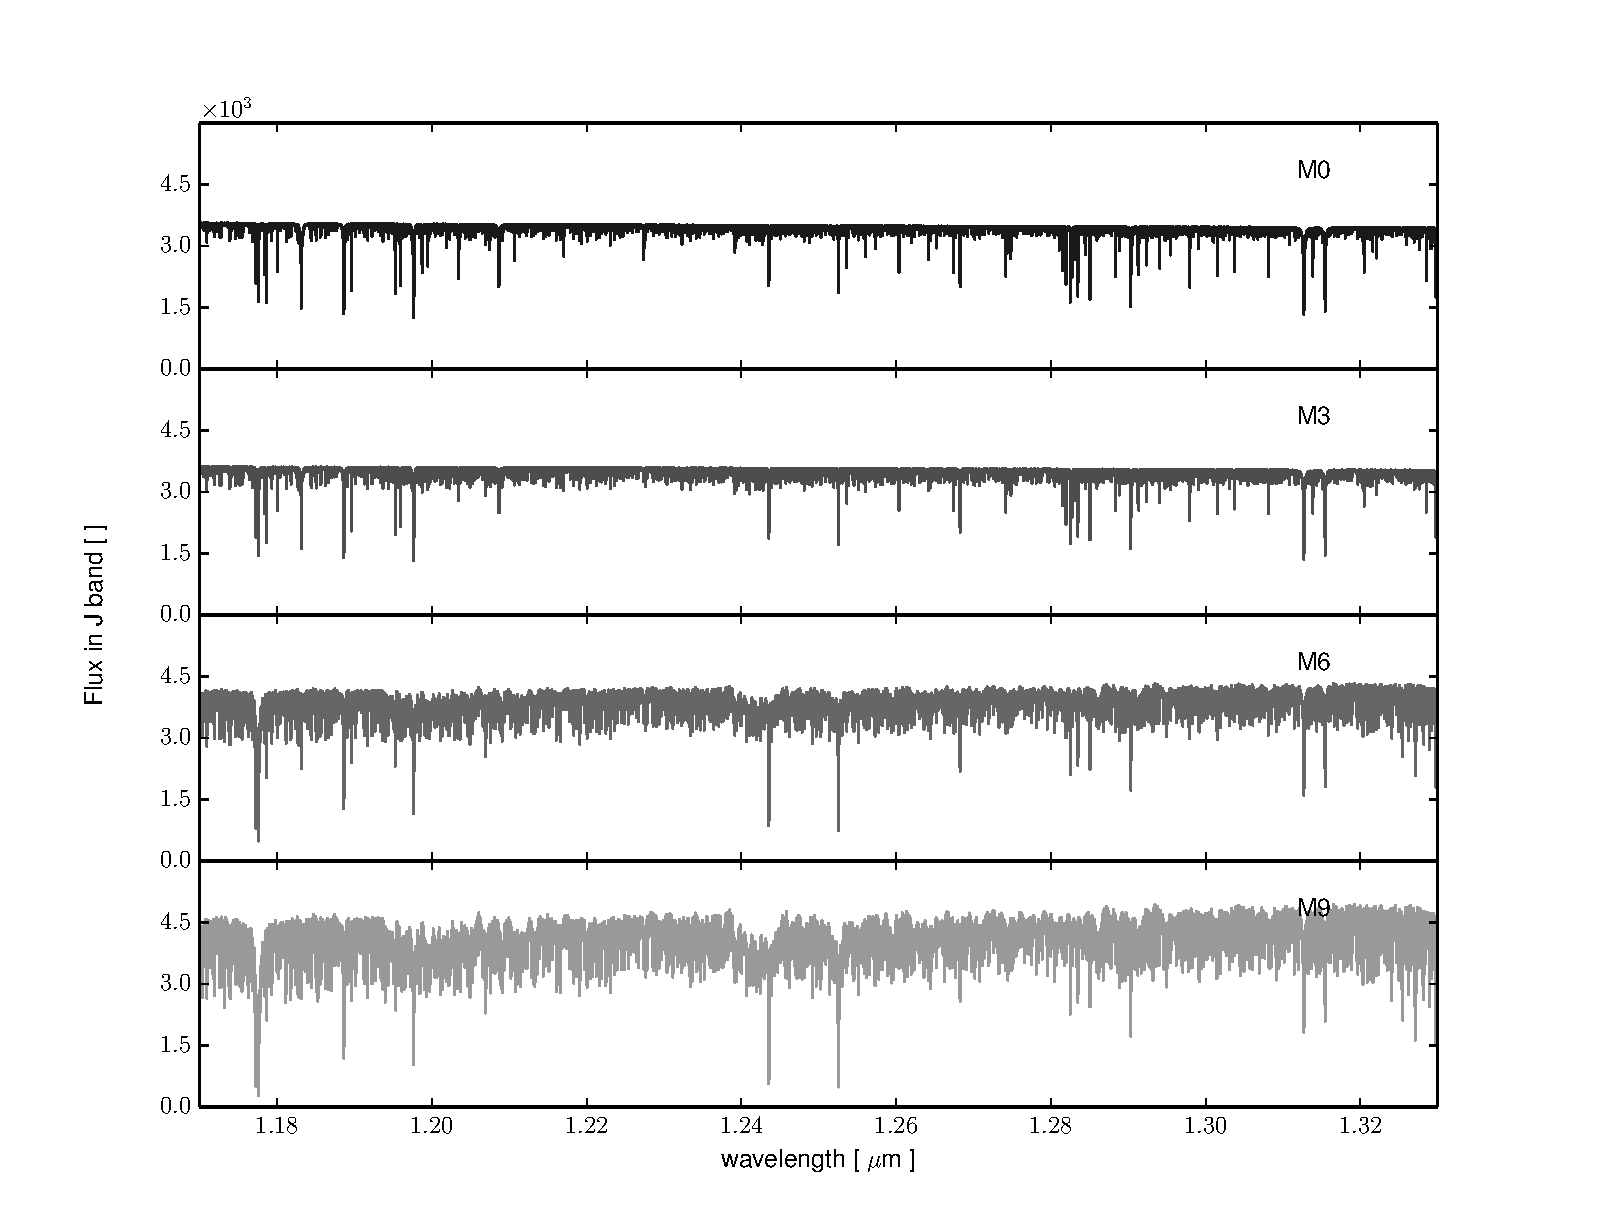
\includegraphics[width=0.78\linewidth]{figures/information-content/figueria_2016_figures/Jband}
    \caption[Spectral fluxes in the \emph{Z}-band and \emph{J}-band.]{Flux as a function of wavelength in the \emph{Z}-band (top) and \emph{J}-band (bottom) for the \Vsini{}=1.0\kmps{} and spectral types {M0}, {M3}, {M6}, and {M9} (\textit{top} to \textit{bottom} panels), when seen at a resolution at 100\,000.
        Flux units are arbitrary.
        Reproduced from~\citet{figueira_radial_2016}.}
    \label{fig:z_and_j_spectra}
\end{figure}

This work begins to reveal how the spectral parameters \Logg{} and \feh{} begin to affect the {RV} precision obtained.
It shows that there are some fairly consistent trends at the longer wavelength bands, but in the \emph{Z}-, \emph{H}-, and \emph{J}-bands the effect clearly also depends on the spectral type.
This is just the first look into the relationships between \feh{} and \Logg{} in relation to the spectral quality.

With the possibility to simply compute the quality and precision of a large range of synthetic spectral parameters, a comparison of spectral quality over all synthetic spectra or just all in the M-dwarf temperature range, may help solidify or extend the trends observed here. For example, this work has yet assessed the spectral quality when both \feh{} and \Logg{} are changed together.

In the context of selecting M-dwarf targets for {RV} measurements, if the goal is to achieve a high spectral quality, then it follows from \cref{fig:logg_metalicity_deviations} that generally for {M0}-M3 spectral types, and in the \emph{H}- and \emph{K}-band, an observation of a metal-rich (\feh{}>0) M-dwarf with a lower \Logg{} value would have a higher spectral quality.
In practise, the spectral quality is only one component to the precision, and probably the more important, and observer adjustable,  contribution to spectral precision is the number of photons counted (or the \snr{} achieved).
For cool {M6} and {M9} spectral types this is important as longer exposure times are needed to achieve a similar \snr{} level due to their lower luminosity.


\section{{SPIRou} and {NIRPS} {ETC}}
\label{sec:spirou_nirps_etc}
Having \eniric{} as a tool to calculate {RV} precisions efficiently lead to contributions to the Exposure Time Calculators (ETC) for both the {SPIRou} and {NIRPS} spectrographs.
In this way the expected radial velocity precision of the targets can be estimated and provided to those preparing to observe with these spectrographs.
The calculations were performed at the individual request of both instruments.

In September 2017 \eniric{} was used to provide precision calculations for the {SPIRou} ETC\footnote{\href{http://www.cfht.hawaii.edu/Instruments/SPIRou/SPIRou_etc.php}{\url{http://www.cfht.hawaii.edu/Instruments/SPIRou/SPIRou\_etc.php}}.}.
These were the same spectral parameters as~\citet{figueira_radial_2016} except with the precisions for each band referenced to {\snr{}=100} in its own band.
The modification of \cref{subsec:snr_scaling} was made to fulfil this request.
These values are given in \cref{tab:spirou_precisions}.

In May 2018 \eniric{} was used to provide precision calculations for the {NIRPS} {ETC}.
This extended the spectral range from {M0}, {M3}, {M6}, {M9} at 3900, 3500, 2800, 2600\K{} respectively, to all temperatures between 2500\K{} and 4000\K{} inclusively.
This provides a finer resolution coverage over the M spectral type, allowed by the {PHOENIX-ACES} library.
Instrumental resolutions of 75\,000 and 100\,000 were requested to match the {NIRPS} instrument.
The \Logg{}, metallicity, and sampling rate remained at the~\citet{figueira_radial_2016} levels of 4.5, 0.0 and 3.0 respectively.
Precisions were provided for \snr{} of 100 relative to the \emph{J}- and \emph{H}-bands as well as to each band individually.
Artigua (\emph{priv.\ comm.} 2018) suggested the truly relevant values would be the \snr{} in \emph{H}-band for {NIRPS} instrument.
The values calculated for {NIRPS} are given in \cref{tab:nirps_precisions}.

The resulting tables, along with the command line incantations to produce them are detailed in \cref{appendix:nir_prec_amendment}.

\clearpage